
\documentclass[master]{thesis-uestc}

\title{数字相控阵单脉冲测向方法研究}{The Research on Monopulse estimation with 
Digital Phased Array}

\author{邓宇昊}{Yuhao Deng}
\advisor{谢菊兰\chinesespace 副教授}{Dr. Julan Xie}
\school{信息与通信工程学院}{School of Information and Communication Engineering}
\major{信号与信息处理}{Signal and Information Processing}
\studentnumber{201821011229}

\begin{document}

\makecover

\begin{chineseabstract}
这是摘要

……

\chinesekeyword{关,键,词}
\end{chineseabstract}

\begin{englishabstract}
This is abstract.

\englishkeyword{key, words}
\end{englishabstract}

\thesistableofcontents

\thesischapterexordium

\section{研究工作的背景与意义}
计算电磁学方法\citing{wang1999sanwei, liuxf2006, zhu1973wulixue, chen2001hao, gu2012lao, feng997he}
从时、频域角度划分可以分为频域方法与时域方法两大类。频域方法的研究开展较早,
目前应用广泛的包括:矩量法(MOM)\citing{xiao2012yi,zhong1994zhong}及其快速算法多层快速多极子(MLFMA)
\citing{clerc2010discrete}方法、有限元(FEM)\citing{wang1999sanwei,zhu1973wulixue}方法、
自适应积分(AIM)\citing{gu2012lao}方法等,
这些方法是目前计算电磁学商用软件\footnote{脚注序号“\ding{172},……,\ding{180}”的字体是“正文”,不是“上标”,
序号与脚注内容文字之间空1个半角字符,脚注的段落格式为:单倍行距,段前空0磅,段后空0磅,悬挂缩进1.5字符;
中文用宋体,字号为小五号,英文和数字用Times New Roman字体,字号为9磅;
中英文混排时,所有标点符号(例如逗号“,”、括号“()”等)一律使用中文输入状态下的标点符号,
但小数点采用英文状态下的样式“.”。}(例如:FEKO、Ansys 等)的核心算法。
由文献\cite{feng997he,clerc2010discrete,xiao2012yi}可知

\section{单脉冲方法的国内外研究历史与现状}
时域积分方程方法的研究始于上世纪60 年代,

\section{本文的主要贡献与创新}
本论文以时域积分方程时间步进算法的数值实现技术、后时稳定性问题以及两层平面波加速算法为重点研究内容,主要创新点与贡献如下:

\section{本论文的结构安排}
本文的章节结构安排如下:

\chapter{相控阵单脉冲测向基本理论}
本章将介绍相控阵单脉冲测向的基本原理,首先给出几种相控阵的接收信号模型,然后介绍波束形成技术,
最后给出三种常用的传统单脉冲测向方法。在本章中,所有入射信号都假设为远场窄带信号,
构成阵列的所有天线均为完全一致且理想的全向天线,没有幅相误差,不考虑阵元间互耦。

\section{相控阵接收信号模型}
依据相控阵阵元天线的排布方式,我们可以将相控阵划分为规则阵和共形阵。
前者主要有均匀线阵、均匀面阵和均匀圆阵,而后者代指天线排布没有特定几何规律的“一般”阵列。
对于远场窄带信号,其一般表达式为$s(t)=A(t)\exp\left[-j\left(2\pi ft+\varphi(t)\right)\right]$,
其中$A(t)$为入射信号的振幅,$\varphi(t)$为初相位。
对于入射信号波程差引起的短时延$\tau$,远场窄带信号有式\eqref{approx}成立。
\begin{equation}\label{approx}
\begin{aligned}
    A(t-\tau) &\approx A(t) \\
    \varphi(t-\tau) &\approx \varphi(t)
\end{aligned}
\end{equation}
因此我们可以忽略时延$\tau$对信号振幅和初相位的影响。
若假设阵列由$M$个阵元组成,则可以得到第$m$个阵元相对于阵列参考点的输出
$s(t)\exp\left(-j2\pi f\tau_m\right)$。
我们进一步将$M$个阵元的输出信号重写为向量形式$\bm{y}$,并且假设每个阵元的噪声都是独立同分布的
零均值高斯白噪声,即$\bm{n}\sim\mathcal{N}\left(0,\sigma^2_n\bm{I}\right)$。
利用上述假设,相控阵接收信号模型可以被表述为式\eqref{data_model}。
\begin{equation}\label{data_model}
    \begin{aligned}
        \bm{y} = s(t)\bm{a} + \bm{n}
    \end{aligned}
\end{equation}
式\eqref{data_model}中,向量$\bm{a}\in\mathbb{C}^{M\times1}$称为导向向量,
是一个与信号入射方向以及阵元排布方式有关的向量。
在接下来的小节中,我们将讨论不同阵列的导向向量。

\subsection{均匀线阵}
均匀线阵是指阵列的所有阵元等间距分布在一条线(如$x$轴)上的阵列。
在本节中我们设相邻两阵元的间距为$d$。
若考虑一远场窄带信号$s(t)$,以俯仰角$\phi$入射到由$M$个阵元组成的均匀线阵上,
如图\ref{ULA}所示。
\begin{figure}[h]
\includegraphics[scale=0.8]{pic/ULA.pdf}
\caption{均匀线阵接收信号模型}
\label{ULA}
\end{figure}

对于均匀线阵,俯仰角$\phi$的定义域通常为$\phi\in\left(-90^\circ,90^\circ\right)$。
设阵列参考点为$O$,即左起第一个阵元。由几何关系我们可以得知,第$m$个阵元相对于参考点的波程差为
$(m-1)d\sin\phi$,因此我们可以得到第$m$个阵元相对于参考点的时延$\tau_m$。
\begin{equation}\label{time_delay}
    \begin{aligned}
    \tau_m = \frac{(m-1)d\sin\phi}{c}
    \end{aligned}
\end{equation}
利用式\eqref{time_delay},均匀线阵的导向向量可以由式\eqref{sv_ULA}表出。
\begin{equation}\label{sv_ULA}
    \begin{aligned}
        \bm{a}(\phi) = 
        \left[
        1,
        \exp\left(j\frac{2\pi d\sin\phi}{\lambda}\right),
        \cdots,
        \exp\left(j\frac{2\pi(M-1)d\sin\phi}{\lambda}\right)
        \right]^T
    \end{aligned}
\end{equation}

在均匀线阵中,要求相邻两阵元间距$d\leq\lambda/2$,否则会造成相位混叠,进而影响单脉冲测向。

\subsection{均匀面阵}
均匀面阵是指所有阵元分布在一个矩形平面如$xOy$平面上,所有阵元共面。
其$x$轴方向上的任意两相邻阵元间距均为$d_x$,
$y$轴方向上的任意两相邻阵元间距均为$d_y$,如图\ref{URA}所示。
\begin{figure}[h]
\includegraphics[scale=0.8]{pic/URA.pdf}
\caption{均匀面阵接收信号模型}
\label{URA}
\end{figure}

图\ref{URA}中,期望信号$s(t)$以方位角$\theta$和俯仰角$\phi$入射到该均匀面阵上。
一般情况下,方位角$\theta$的定义域取$\theta\in\left[-180^\circ,180^\circ\right)$,
俯仰角的定义域取$\phi\in\left[0^\circ,90^\circ\right)$。
若假设该均匀面阵共有$M \times N$个阵元,其中$x$轴方向上$M$行,$y$轴方向上$N$列。
依照几何关系依旧可以得到第$(m,n)$个阵元相对于参考点的波程差,进一步得到时延$\tau_{m,n}$。
\begin{equation}\label{URA_time_delay}
    \begin{aligned}
        \tau_{m,n} = 
        \frac{(m-1)d_x\sin\phi\cos\theta + (n-1)d_y\sin\phi\sin\theta}{c}
    \end{aligned}
\end{equation}

因此可以构造一个$M \times N$的矩阵$\bm{S}$,它的第$m$行,
第$n$列元素是第$(m,n)$个阵元相对于参考点的相位差,
即\eqref{URA_phase_delay}式。
\begin{equation}\label{URA_phase_delay}
    \begin{aligned}
        \left[\bm{S}\right]_{m,n} = 
        \exp\left(j\frac{2\pi}{\lambda}
                  \left[(m-1)d_x\sin\phi\cos\theta + (n-1)d_y\sin\phi\sin\theta\right]\right)
    \end{aligned}
\end{equation}
我们利用上一节中均匀线阵的导向向量形式\eqref{sv_ULA},
可以将矩阵$\bm{S}$重写为\eqref{sv_mat_URA}式。
\begin{equation}\label{sv_mat_URA}
    \begin{aligned}
        \bm{S}(\theta,\phi) = \bm{a}_x\bm{a}^T_y
    \end{aligned}
\end{equation}
式\eqref{sv_mat_URA}中,向量$\bm{a}_x\in\mathbb{C}^{M\times1}$和$\bm{a}_y\in\mathbb{C}^{N\times1}$
分别为$x$轴方向和$y$轴方向上均匀线阵形式的导向向量,
其定义由式\eqref{subsv_URA}表出。
\begin{subequations}\label{subsv_URA}
    \begin{align}
        \left[\bm{a}_x\right]_{m} &= 
        \exp\left(j\frac{2\pi(m-1)d_x\sin\phi\cos\theta}{\lambda}\right)
        \\
        \left[\bm{a}_y\right]_{n} &= 
        \exp\left(j\frac{2\pi(n-1)d_y\sin\phi\sin\theta}{\lambda}\right)
    \end{align}
\end{subequations}

最后,我们将矩阵$\bm{S}$按列优先重排得到均匀面阵的导向向量$\bm{a}\in\mathbb{C}^{MN\times1}$。
\begin{equation}\label{sv_URA}
    \begin{aligned}
        \bm{a}(\theta,\phi) = \text{vec}\left(\bm{a}_x\bm{a}_y^T\right)
    \end{aligned}
\end{equation}
上式中,$\text{vec}(\cdot)$表示按列优先重排向量。

\subsection{均匀圆阵}
均匀圆阵指阵列中的所有阵元都均匀分布在一个半径为$R$的圆上,且所有阵元共面。
通常情况下,以圆心$O$作为阵列参考点,如图\ref{UCA}所示。
\begin{figure}[h]
\includegraphics[scale=0.8]{pic/UCA.pdf}
\caption{均匀圆阵接收信号模型}
\label{UCA}
\end{figure}

假设一期望信号以方位角$\theta$,俯仰角$\phi$入射到$M$个阵元组成的均匀圆阵上。
由于$M$个阵元均分圆周,即任意两相邻两阵元的圆弧长相等,
因此我们可以得到第$m$个阵元的坐标$\bm{r}_m$。
\begin{equation}\label{pos_UCA}
    \begin{aligned}
        \bm{r}_m = \left[
            R\cos\varphi_m,
            R\sin\varphi_m,
            0
           \right]^T 
    \end{aligned}
\end{equation}
式\eqref{pos_UCA}中,$\varphi_m$表示第$m$个阵元与$x$轴的夹角,
我们限定其定义域为$\varphi_m\in\left[-\pi,\pi\right)$,
然后给出$\varphi_m$的表达式\eqref{angle_UCA}。
\begin{equation}\label{angle_UCA}
    \begin{aligned}
        \varphi_m = 2\pi\frac{-(M-1)/2+m-1}{M}
    \end{aligned}
\end{equation}

利用$\bm{r}_m$和入射信号角度可以计算出第$m$个阵元相对于参考点$O$的波程差,
进一步得到均匀圆阵导向向量$\boldsymbol{a}\in\mathbb{C}^{M\times1}$。
该导向向量的元素由式\eqref{sv_UCA}表出。
\begin{equation}\label{sv_UCA}
    \begin{aligned}
        \left[\bm{a}(\theta,\phi)\right]_m 
        &= 
        \exp\left[j\frac{2 \pi R}{\lambda}
                  \left(
                  \cos\varphi_m\sin\phi\cos\theta + 
                  \sin\varphi_m\sin\phi\sin\theta
                  \right)
            \right]
            \\
        &=    
            \exp\left[
            j\frac{2\pi R}{\lambda}\sin\phi
            \cos\left(\theta-\varphi_m\right)
            \right]
    \end{aligned}
\end{equation}

\subsection{共形阵}
共形阵没有特定的几何规则,导向向量往往与参考点的选取有关。
考虑一个远场窄带信号$s(t)$,以方位角$\theta$和俯仰角$\phi$入射到由$M$个阵元组成的共形阵上,
如图\ref{conformal_array}所示。
\begin{figure}[h]
\includegraphics[scale=0.8]{pic/conformal_array.pdf}
\caption{共形阵接收信号模型}
\label{conformal_array}
\end{figure}
假设共形阵的参考点为坐标原点$O$,第$m$个阵元的位置向量为$\bm{r}_m=\left[x_m,y_m,z_m\right]^T$。
入射信号的方向向量由式\eqref{dir_vec}给出。
\begin{equation}\label{dir_vec}
    \bm{\epsilon}_p=-\left[\sin\phi\cos\theta,
                                   \sin\phi\sin\theta,
                                   \cos\phi\right]^T
\end{equation}
因此,我们可以得到第$m$个阵元相对于参考点$O$的相位差$u_m$
\begin{equation}\label{delay}
    \begin{aligned}
        u_m = \exp\left(-j\frac{2\pi}{\lambda}\bm{r}_m^T\bm{\epsilon}_p\right)
    \end{aligned}
\end{equation}
进一步得到共形阵的导向向量$\bm{a}\in\mathbb{C}^{M\times1}$。
\begin{equation}\label{sv}
    \begin{aligned}
        \bm{a}\left(\theta,\phi\right) = 
        \left[\exp\left(-j\frac{2\pi}{\lambda}\bm{r}_1^T\bm{\epsilon}_p\right),
              \exp\left(-j\frac{2\pi}{\lambda}\bm{r}_2^T\bm{\epsilon}_p\right),
              \cdots,
              \exp\left(-j\frac{2\pi}{\lambda}\bm{r}_M^T\bm{\epsilon}_p\right)\right]^T
    \end{aligned}
\end{equation}

式\eqref{sv}是相控阵导向向量的一般表达式,前几个小节中的规则阵列导向向量均可以使用式\eqref{sv}表出。

\section{波束形成技术}
波束形成技术是一种相控阵的空域处理技术,其主要目的是让阵列形成指向,
使得阵列接收信号功率集中于目标方向附近,同时抑制非目标方向的干扰。
波束形成的主要原理是通过对阵列中的各个阵元的输出信号进行加权补相并求和,
使得目标方向上的相位叠加增强,而非目标方向上的相位叠加相消。
让阵列对准目标方向,形成一个指向目标的“波束”,同时对于其余方向上的干扰以及噪声有一定抑制。
在本章中,我们将以半波长间距的均匀线阵为例,分析波束形成的原理和一般过程。

\subsection{MVDR波束形成方法}
MVDR方法即最小方差无失真响应方法,本节我们将以单信源入射均匀线阵为例分析其原理。
考虑一期望信号$s(t)$由方向$\phi_0$入射到$M$阵元的均匀线阵上,
由式\eqref{data_model}知$M$个阵元的输出记为向量$\bm{y}$。
现假设有一$M$个抽头的空域滤波器,其权向量为$\bm{w}\in\mathbb{C}^{M\times1}$。
阵列的输出信号通过该滤波器的输出为$z$,由式\eqref{filter_model}表出。
\begin{equation}\label{filter_model}
    \begin{aligned}
    z = \bm{w}^H\bm{y} = \bm{y}^T\bm{w}^*
    \end{aligned}
\end{equation}
上式中,$\cdot^*$表示转置。
利用式\eqref{filter_model}可以得到该滤波器输出的平均功率$\sigma^2$。
\begin{equation}\label{mvdr_var}
    \begin{aligned}
    \sigma^2 &= E\left\{|z|^2\right\} \\
             &= E\left\{\bm{w}^H\bm{y}\bm{y}^H\bm{w}\right\} \\
             &= \bm{w}^H\bm{Q}\bm{w}
    \end{aligned}
\end{equation}
式\eqref{mvdr_var}中,矩阵$\bm{Q}=E\left\{\bm{y}\bm{y}^H\right\}$
是干扰叠加噪声(即不含有期望信号)的协方差矩阵。

由于期望信号的入射方向是$\phi_0$,利用式\eqref{data_model}和式\eqref{filter_model}可知,
理想情况下(不考虑噪声)滤波器的输出应该是式\eqref{filter_obj}中的$z_0$。
\begin{equation}\label{filter_obj}
    \begin{aligned}
    z_0 = \bm{w}^H\bm{y}(\phi_0) = \bm{w}^H\bm{a}(\phi_0)s(t)
    \end{aligned}
\end{equation}
由于我们要求空域滤波器在目标方向上无失真的通过,因此我们可以令约束条件为式\eqref{constraint}。
\begin{equation}\label{constraint}
    \begin{aligned}
    \bm{w}^H\bm{a}(\phi_0) = 1
    \end{aligned}
\end{equation}
同时,为了抑制其他方向上的干扰和噪声,我们还需要使得滤波器输出的平均功率最小,
因此,该波束形成问题可以表述为一个带约束条件的优化问题,如式\eqref{MVDR_obj}所示。
\begin{equation}\label{MVDR_obj}
    \begin{aligned}
    &\min_\bm{w} ~ \bm{w}^H\bm{Q}\bm{w} \\
    &\text{s.t.} ~ \bm{w}^H\bm{a}(\phi_0) = 1
    \end{aligned}
\end{equation}

我们可以用拉格朗日乘子法求解该问题,首先构造代价函数$J(\bm{w})$。
\begin{equation}
    \begin{aligned}
    J(\bm{w}) = \bm{w}^H\bm{Q}\bm{w} + \mu\left(\bm{w}^H\bm{a}(\phi_0)-1\right)
    \end{aligned}
\end{equation}
然后对代价函数$J(\bm{w})$求梯度,并令其等于$\textbf{0}$向量。
\begin{equation}\label{cost_grad}
    \begin{aligned}
    \nabla J(\bm{w}) = 2\bm{Q}\bm{w} - 2\bm{a}(\phi_0) = \textbf{0}
    \end{aligned}
\end{equation}
求解式\eqref{cost_grad}我们可以得到$\bm{w}$的解。
\begin{equation}\label{w_mu}
    \begin{aligned}
    \bm{w} = \mu\bm{Q}^{-1}\bm{a}(\phi_0)
    \end{aligned}
\end{equation}
注意式\eqref{w_mu}中,只要干扰信号是非相干的,那么协方差矩阵$\bm{Q}$一定可逆。
本小节中只存在一个期望信号,无干扰,而我们假设每个阵元的噪声都是独立同分布的高斯白噪声,
此时矩阵$\bm{Q}$一定可逆。
然后将式\eqref{w_mu}带入式\eqref{constraint},我们可以得到拉格朗日乘子$\mu$。
\begin{equation}\label{larg_arg}
    \begin{aligned}
    \mu = \frac{1}{\bm{a}^H(\phi_0)\bm{Q}^{-1}\bm{a}(\phi_0)}
    \end{aligned}
\end{equation}

最后,我们将式\eqref{larg_arg}带入\eqref{w_mu},得到MVDR权向量的最优解$\bm{w}_o$。
\begin{equation}\label{w_solve}
    \begin{aligned}
    \bm{w}_o = \frac{\bm{Q}^{-1}\bm{a}(\phi_0)}{\bm{a}^H(\phi_0)\bm{Q}^{-1}\bm{a}(\phi_0)}
    \end{aligned}
\end{equation}

MVDR方法要求干扰源的个数小于或等于$M-1$,否则将会导致协方差矩阵$Q$的退化,
我们将$M-1$称为阵列的自由度。对于满足各态历经性的信号$\bm{y}$,我们可以用时间平均估计出其统计平均,
并由此得到协方差矩阵的估计量。

\subsection{LCMV波束形成方法}
MVDR方法的局限性在于,它只有一组约束条件,即期望信号无失真通过。
当阵列需要在多个方向上形成波束,或者在指定方向上形成零点抑制干扰时,MVDR方法就无法胜任这一工作了。
因此在本小节中,我们将介绍一种线性约束最小方差方法,即LCMV方法。

LCMV方法的基本原理相同,我们仍旧需要使空域滤波器的平均输出功率最小,但此时约束条件发生了改变。
假设一个$M$阵元的均匀线阵,
若需要形成$L$个波束,在$\phi_1,\phi_2,\cdots,\phi_L$方向上保持接收信号的单位增益,
同时需要形成$P$个零陷,在$\phi_{L+1},\phi_{L+2},\cdots,\phi_{L+P}$方向上形成零陷用于抑制干扰。
此时,我们可以将多个约束条件写成矩阵乘法的形式,如式\eqref{LCMV_constraint}所示。
\begin{equation}\label{LCMV_constraint}
    \begin{aligned}
        \bm{C}^H\bm{w} = \bm{f}
    \end{aligned}
\end{equation}
上式中,矩阵$\bm{C}\mathbb{C}^{M\times(L+P)}$称为约束矩阵,向量$\bm{f}\in\mathbb{C}^{(L+P)\times1}$
为对应的约束向量。对于上述约束条件,我们可以将其表述为式\eqref{costraint_mat_vec}。
\begin{subequations}\label{costraint_mat_vec}
    \begin{align}
        \bm{C} &= \left[\bm{a}(\phi_1), \cdots, \bm{a}(\phi_L), 
                        \bm{a}(\phi_{L+1}), \cdots, \bm{a}(\phi_{L+P})\right]
        \\
        \bm{f} &= \left[1, \cdots, 1, 0, \cdots, 0\right]^T
    \end{align}
\end{subequations}
类似于MVDR方法,我们依旧可以将该问题表述为一个带约束条件的优化问题,即式\eqref{LCMV_obj}。
\begin{equation}\label{LCMV_obj}
    \begin{aligned}
        &\min_\bm{w} ~ \bm{w}^H\bm{Q}\bm{w} \\
        &\text{s.t.} ~ \bm{C}^H\bm{w} = \bm{f}
    \end{aligned}
\end{equation}
同样利用拉格朗日乘子法构造代价函数,并令其梯度为$\textbf{0}$向量,然后解得
\begin{equation}\label{LCMV_w_mu}
    \begin{aligned}
    \bm{w} = \frac{1}{2}\bm{Q}^{-1}\bm{C}\bm{\mu}
    \end{aligned}
\end{equation}
注意,上式中的向量$\bm{\mu}$是拉格朗日乘子,然后将式\eqref{LCMV_w_mu}带入式\eqref{LCMV_constraint}中
得到
\begin{equation}\label{LCMV_mu}
    \begin{aligned}
        \bm{\mu} = 2\left(\bm{C}^H\bm{Q}^{-1}\bm{C}\right)^{-1}\bm{f}
    \end{aligned}
\end{equation}
最后将式\eqref{LCMV_mu}带入式\eqref{LCMV_w_mu}得到LCMV的最优权向量$\bm{w}_o$,由式\eqref{LCMV_w_opt}表出。
\begin{equation}\label{LCMV_w_opt}
    \begin{aligned}
        \bm{w}_o = \bm{Q}^{-1}\bm{C}\left(\bm{C}^H\bm{Q}^{-1}\bm{C}\right)^{-1}\bm{f}
    \end{aligned}
\end{equation}

与MVDR方法一样,LCMV也存在阵列自由度$M-1$,约束条件的个数$L+P \leq M-1$,
否则将会引起协方差矩阵$Q$的退化。实际上,MVDR方法是LCMV方法的一种特殊情况,
即约束条件的个数只有一个。LCMV方法给出了一种广义形式,在后续的自适应单脉冲测向中,
我们还会用到该方法。

\section{传统单脉冲方法}
在上一节中,我们假设波束形成的方向$\phi_0$和期望信号的真实方向$\phi_s$是一致的。
但在实际情况中,由前端处理得到的波束指向角$\phi_0$并不一定等于$\phi_s$,
往往还相差了一个较小的角度$\pm\Delta\phi$,但真实角度$\phi_s$一般处于波束的$3$dB宽度以内。
因此,我们需要一种方法在已知波束指向角的情况下测量期望信号的真实方向。
单脉冲测向方法就是用于解决该问题的。通常情况下,
单脉冲测向方法需要在阵列的输出端分别形成和波束与差波束,
其中和波束要求在波束指向处形成主瓣增益,而差波束则需要在波束指向处形成零陷。
然后利用单脉冲比即差和比估计出期望信号方向与波束指向间的差值$\Delta\phi$,
进一步得到期望信号的真实方向。

传统的单脉冲测向方法主要由三种,分别是半阵法、加权法和和差比幅法,
我们在接下来的小节中将会依次结束这三种方法。
值得注意的是,这三种方法都是静态非自适应方法,不依赖于干扰叠加噪声的统计特性。
其中只有加权测向方法可以抑制旁瓣干扰,并且三种方法都无法抑制主瓣干扰。
三种方法的主要区别在于和波束与差波束的形成方式不同。

\subsection{半阵测向}
半阵测向方法利用阵列的几何对称性来构造和差波束权向量,
因此主要用于均匀线阵和均匀面阵这种拥有范德蒙德结构导向向量的规则阵列。
本节中我们以线阵为例,解析半阵测向的原理和过程。

首先考虑一$2M$阵元的均匀线阵,阵元间距为$d$,波束指向为$\phi_0$。
由于和波束要求在波束指向$\phi_0$处形成主瓣增益,
因此我们可以取和波束权$\bm{w}_\Sigma$为指向$\phi_0$处的导向向量。
\begin{equation}\label{semi_w_s}
    \begin{aligned}
        \bm{w}_\Sigma = \bm{a}(\phi_0)
    \end{aligned}
\end{equation}
利用均匀线阵的对称性,我们取差波束$\bm{w}_\Delta$为
\begin{equation}\label{semi_w_d}
    \begin{aligned}
        \bm{w}_\Delta = [\overbrace{-1,\cdots,-1}^M,
                              \overbrace{1,\cdots,1}^M]^T \odot \bm{a}(\phi_0)
    \end{aligned}
\end{equation}
式\eqref{semi_w_d}中,$\odot$表示Hadamard积。
假设期望信号的入射方向为$\phi_s$,其导向向量为$\bm{a}(\phi_s)$,和波束输出为$\Sigma(\phi_s)$,
差波束输出为$\Delta(\phi_s)$。
\begin{subequations}\label{delta_and_sigma}
    \begin{align}
        \Sigma(\phi_s)  = \bm{w}_\Sigma^H\bm{a}(\phi_s)
                       &= \sum_{m=1}^{2M}\exp\left[
                                           j\frac{2\pi(m-1)d}{\lambda}(\sin\phi_s-\sin\phi_0)
                                           \right]
        \\
        \Delta(\phi_s)  = \bm{w}_\Delta^H\bm{a}(\phi_s)
                       &= \sum_{m=M+1}^{2M}\exp\left[
                                             j\frac{2\pi(m-1)d}{\lambda}(\sin\phi_s-\sin\phi_0)
                                             \right] \\
                       \nonumber
                       &- \sum_{m=1}^{M}\exp\left[
                                             j\frac{2\pi(m-1)d}{\lambda}(\sin\phi_s-\sin\phi_0)
                                             \right]
    \end{align}
\end{subequations}
为便于化简,我们设波束$P$为
\begin{equation}\label{semi_pattern}
    \begin{aligned}
        P = \sum_{m=1}^{M}\exp\left[
                                   j\frac{2\pi(m-1)d}{\lambda}(\sin\phi_s-\sin\phi_0)
                               \right]
    \end{aligned}
\end{equation}
然后将式\eqref{semi_pattern}代入\eqref{delta_and_sigma}得到
\begin{subequations}
    \begin{align}
        \Sigma(\phi_s) &= P\left(
                            \exp\left[
                                   j\frac{2\pi Md}{\lambda}(\sin\phi_s-\sin\phi_0)
                                \right] + 1
                           \right)
                       \\
       \Delta(\phi_s) &= P\left(
                            \exp\left[
                                   j\frac{2\pi Md}{\lambda}(\sin\phi_s-\sin\phi_0)
                                \right] - 1
                           \right)
    \end{align}
\end{subequations}
我们令$u=\sin\phi_s-\sin\phi_0$,利用欧拉公式进一步得到半阵法的单脉冲比$\text{MRC}$
\begin{equation}\label{semi_MRC}
    \begin{aligned}
    \text{MRC} &= \frac{\Delta(\phi_s)}{\Sigma(\phi_s)}
    \\
               &= \frac{\exp\left(j\frac{\pi Md}{\lambda}u\right) -
                        \exp\left(-j\frac{\pi Md}{\lambda}u\right)}
                       {\exp\left(j\frac{\pi Md}{\lambda}u\right) +
                        \exp\left(-j\frac{\pi Md}{\lambda}u\right)}
    \\
               &= j\frac{\sin\left(\pi Mdu/\lambda\right)}{\cos\left(\pi Md u/\lambda\right)}
   \\
               &= j\tan\left(\frac{\pi Md}{\lambda}u\right)          
    \end{aligned}
\end{equation}
在单脉冲测向的场景中,通常假设目标真实方向$\phi_s$与阵列波束指向$\phi_0$相差较小,
由此可知$u=\sin\phi_s-\sin\phi_0$趋近于$0$。
同时由于$\pi M/\lambda$为一有限值,我们可以利用等价无穷小$\tan x \sim x$将单脉冲比$\text{MRC}$
近似为
\begin{equation}\label{MRC_proc}
    \begin{aligned}
    \text{MRC} = j\frac{\pi M}{\lambda}\left(\sin\phi_s-\sin\phi_0\right)
    \end{aligned}
\end{equation}
最后利用Taylor展开式将$\sin\phi_s$在$\phi_0$处展开,
并舍弃二阶及其以上的高次项并带入式\eqref{MRC_proc}得到
\begin{equation}\label{semi_MRC_fin}
    \begin{aligned}
        \text{MRC} = j\frac{\pi Md}{\lambda}\cos\phi_0\left(\phi_s-\phi_0\right)
    \end{aligned}
\end{equation}
若我们取$\Delta\phi=\phi_s-\phi_0$作为偏离角,则可以得到一个关于$\Delta\phi$的线性函数。
接下来我们通过一个例子展示半阵法的和差波束以及单脉冲比曲线(MRC)。

考虑一个$8$阵元的均匀线阵,阵元间距为半波长,若我们设阵列波束指向$\phi_0=0^\circ$,
和波束与差波束如图\ref{semi_sigma_delta}所示,半阵法的单脉冲比曲线如图\ref{semi_MRC}所示。
\begin{figure}[h]
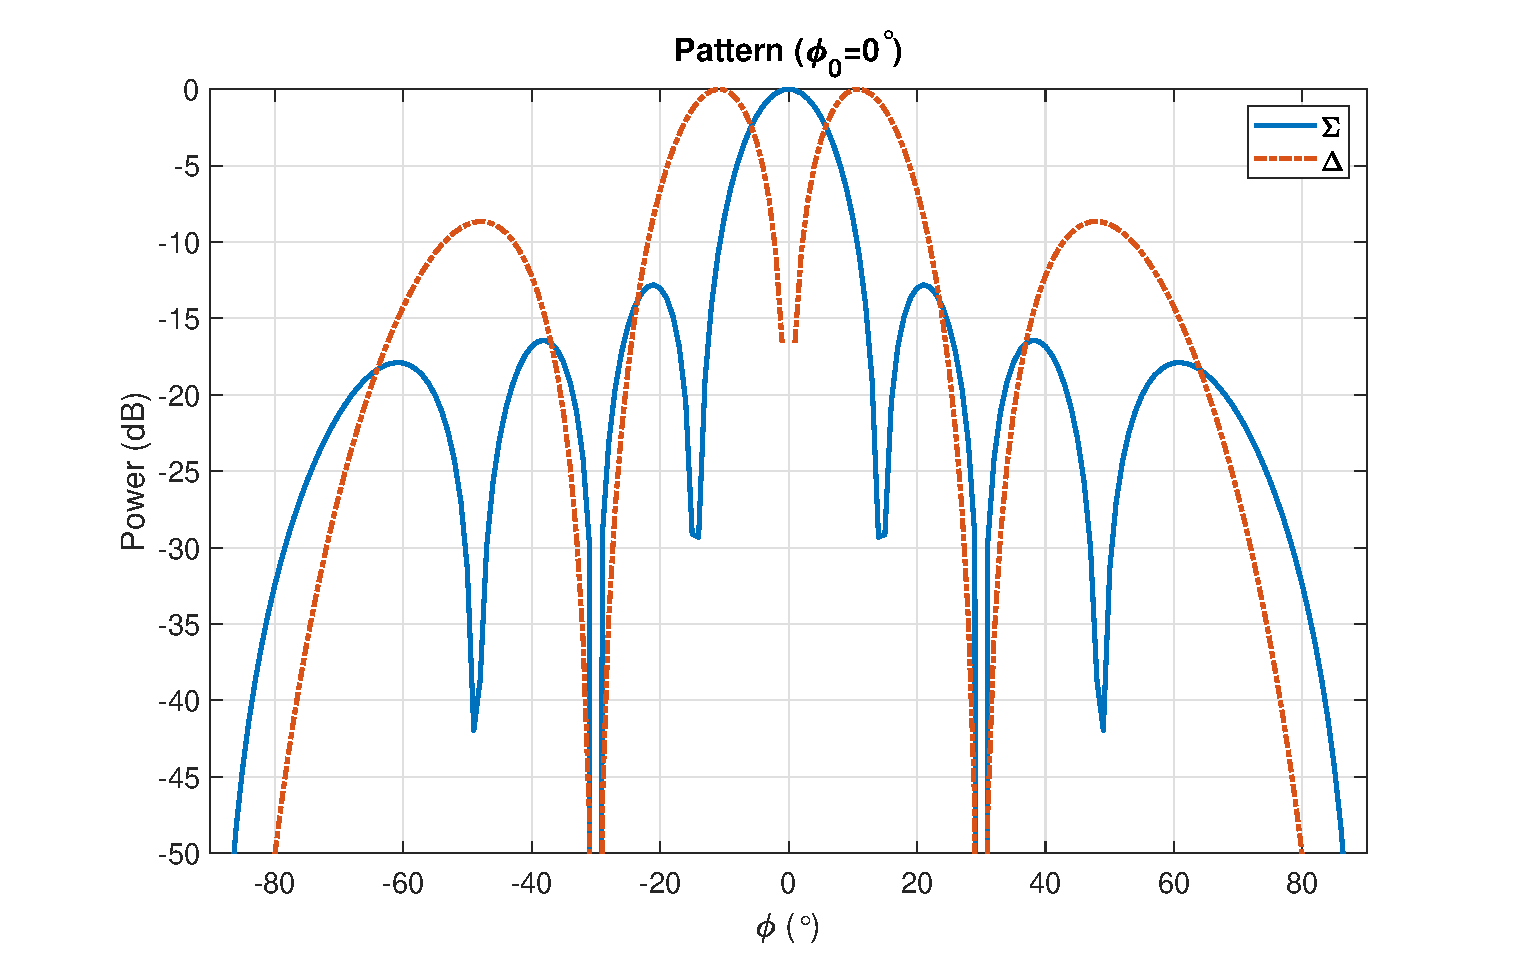
\includegraphics[scale=0.4]{pic/semi_sigma_delta.eps}
\caption{半阵法的和波束$\Sigma$与差波束$\Delta$}
\label{semi_sigma_delta}
\end{figure}

\begin{figure}[h]
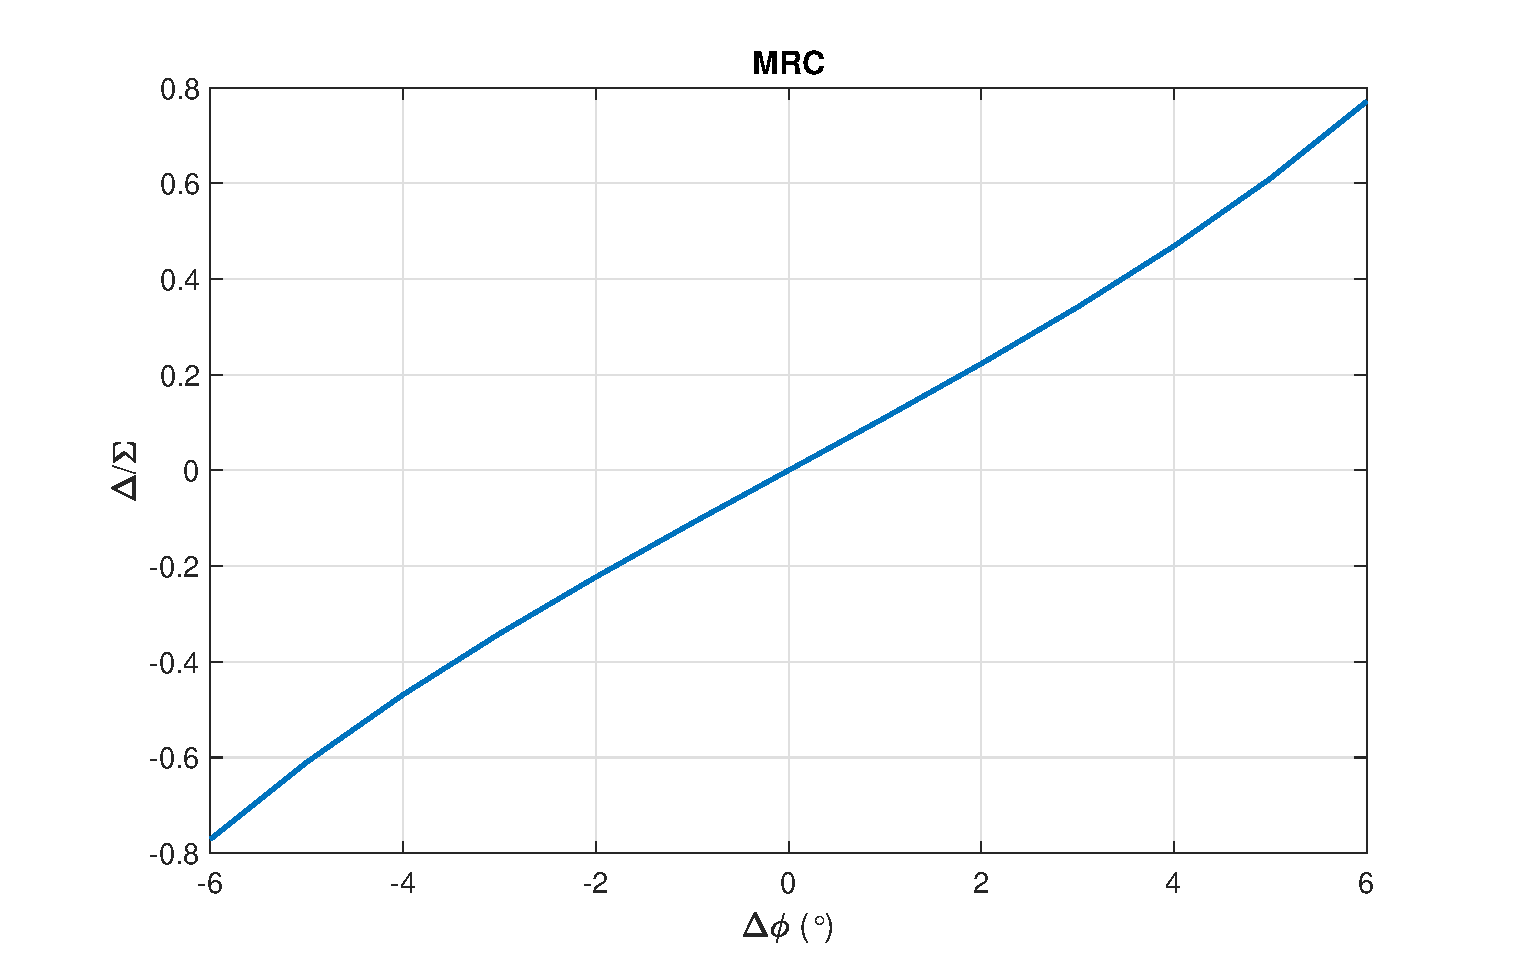
\includegraphics[scale=0.4]{pic/semi_MRC.eps}
\caption{半阵法的单脉冲比曲线}
\label{semi_MRC}
\end{figure}

从图\ref{semi_sigma_delta}中我们可以看出,和波束的主瓣对准了$\phi_0=0^\circ$,
$3$dB衰减边界大致位于$\pm6^\circ$处。差波束在波束指向$\phi_0$处形成了一个较深的零陷,
注意图\ref{semi_sigma_delta}截断了衰减$-50$dB以下的部分。

对于单脉冲曲线图\ref{semi_MRC},我们可以得知当角度$\phi$与波束指向角$\phi_0$较为接近时,
MRC的线性度较好,而在远离波束指向的地方,MRC的线性度较差。
这意味着期望信号的真实方向$\phi_s$偏离波束指向$\phi_0$越多,该方法的测量误差也就越大。

\subsection{加权测向}
半阵法理论过程简明清晰,且MRC有显式的表达式,但其利用了阵列对称性,因此只能用于均匀线阵和均匀面阵。
并且半阵法和差波束权向量直接选取了波束指向的导向向量,因此旁瓣抑制比较低,当测向环境中出现强旁瓣干扰时,
可能会使得该方法失效。因此,另一种设计和差波束权的方式应运而生。

加权法通过对波束指向处的导向向量$\bm{a}(\phi_0)$进行加窗处理,从而设计出一种满足给定旁瓣抑制比的和差波束。
传统的和差波束窗分别是Taylor窗和Bayliss窗,在作者的原文中,
这两种窗分别由圆形孔径和线形孔径天线(模拟天线,非阵列)导出,
而在接下来的内容中,我们将其拓展到均匀线阵上。

首先考虑一个长度为$2a$质地均匀的线形天线孔径,取其中点为参考点$O$,并假设信号以角度$\phi$入射,
如图\ref{linear_aperture}所示。
\begin{figure}[h]
    \includegraphics[scale=0.8]{pic/linear aperture.pdf}
    \caption{线性孔径接收信号模型}
    \label{linear_aperture}
\end{figure}

利用天线理论我们可以得知,线形孔径的响应函数$F(u)$为
\begin{equation}\label{aperture_response}
    \begin{aligned}
        F(u) = \int_{-\pi}^\pi g(x)e^{jux}dx
    \end{aligned}
\end{equation}
上式中,$g(x)$为孔径函数,即线形孔径上每个微元的单位冲激响应函数,
并且由
\begin{subequations}\label{ux_def}
    \begin{align}
        u &= \frac{2a}{\lambda}\sin\phi
        \\
        x &= \frac{\pi}{a}
    \end{align}
\end{subequations}
式\eqref{ux_def}中,$\lambda$为入射信号波长,
$2a$为线形孔径的长度,$\phi$为期望信号入射角度,如图\ref{linear_aperture}所示。
由于和波束要求响应函数为偶函数,因此我们将孔径函数$g(x)$以余弦级数展开得到式\eqref{cos_seq}。
\begin{equation}\label{cos_seq}
    \begin{aligned}
        g_{\Sigma}(x)=\left\{\begin{array}{ll}
        \sum\limits_{l=0}^{\bar{n}-1} B_{l} \cos \left(\mu_{l} x\right), & -\pi \leqslant x \leqslant \pi
        \\
        0, & \text { otherwise }
        \end{array}\right.
    \end{aligned}
\end{equation}
对于线形孔径,我们可以取$\mu_l=l$。
式\eqref{cos_seq}中,$\bar{n}$是我们期望抑制的邻近(主瓣)旁瓣个数。
我们定义对数旁瓣抑制比为$\text{SLL}$
\begin{equation}\label{SLL}
    \begin{aligned}
        \text{SLL} = 20\lg\eta = 10\lg\left(\nu_s^2/\nu_m^2\right)
    \end{aligned}
\end{equation}
式\eqref{SLL}中,$\nu_s^2$和$\nu_m^2$分别为旁瓣功率和主板功率。
在线形孔径的条件下,系数$B_l$由式\eqref{sigma_coeff}表出。
\begin{equation}\label{sigma_coeff}
    \begin{aligned}
        B_{m}=\left\{\begin{array}{ll}
        1, & m=0 \\
        (-1)^{m+1} \frac{\prod\limits_{n=1}^{\bar{n}-1} 1-\frac{m^{2}}{\sigma^{2}\left[A^{2}+(n-1 / 2)^{2}\right]}}{\prod\limits_{n=1 \atop n \neq m}^{\bar{n}-1} 1-\frac{m^{2}}{n^{2}}}, & 0<m<\bar{n} \\
        0, & m \geqslant \bar{n}
        \end{array}\right.
    \end{aligned}
\end{equation}
式\eqref{sigma_coeff}中,$A$和$\sigma^2$由式\eqref{A_sigma}表出。
\begin{subequations}\label{A_sigma}
    \begin{align}
        A &= \operatorname{acosh}\left(10^{-\mathrm{SLL} / 20}\right) / \pi \\
        \sigma^{2} &= \frac{\bar{n}^{2}}{A^{2}+(\bar{n}-1 / 2)^{2}}
    \end{align}
\end{subequations}
利用式\eqref{cos_seq}、\eqref{SLL}、\eqref{sigma_coeff}和\eqref{A_sigma}
我们就可以针对该线形孔径设计出符合要求的和波束权。

现在我们将该结论扩展到均匀线阵上。考虑一个$M$阵元的均匀线阵,阵元间距为半波长。
均匀线阵可以看作是对线形孔径的等间距采样,
此时阵列的输出由式\eqref{aperture_response}变为向量内积,即式\eqref{f_response}。
\begin{equation}\label{f_response}
    \begin{aligned}
        f(\phi) = \bm{g}_\Sigma^H\bm{a}(\phi)
    \end{aligned}
\end{equation}
上式中,$\bm{a}(\phi)$为导向向量,$\bm{g}_\Sigma$为Taylor幅度权向量。
由于均匀线阵是对线形孔径的等间距采样,因此我们可以得到$\bm{g}_\Sigma$的表达式
\begin{equation}\label{g_sigma_vec}
    \begin{aligned}
        \bm{g}_{\Sigma}=\left[g_{\Sigma}\left(x_{1}\right), g_{\Sigma}\left(x_{2}\right), \cdots,                     g_{\Sigma}\left(x_{M}\right)\right]^{T}
    \end{aligned}
\end{equation}
式\eqref{g_sigma_vec}中,$g_\Sigma(x)$为\eqref{cos_seq}中线形孔径函数$g(x)$的余弦展开式。
而$x_1,x_2,\cdots,x_M$表示在区间$\left[-\pi,\pi\right]$中均匀的取$M$个点,
由此得到$M$阵元均匀线阵的Taylor幅度权。

由于Taylor权向量$\bm{g}_\Sigma$为幅度权,不含有相位。因此我们可以通过式\eqref{taylor_w}
得到任意波束指向$\phi_0$的和波束权。
\begin{equation}\label{taylor_w}
    \begin{aligned}
        \bm{w}_\Sigma = \bm{g}_\Sigma \odot \bm{a}(\phi_0)
    \end{aligned}
\end{equation}
上式中,$\odot$表示Hadamard积。

接下来,我们讨论基于Bayliss幅度权的差波束权向量。
与Taylor权类似,均匀线阵的Bayliss权依旧可以从线形孔径模型下扩展得到。
同样,我们考虑一个长度为$2a$的线形孔径,取其中点为参考点$O$,入射信号波长为$\lambda$,角度为$\phi$,
如图\ref{linear_aperture}所示。其响应函数$F(u)$同式\eqref{aperture_response}。
由于差波束要求响应函数为奇函数,因此我们将孔径函数$g(x)$展开为正弦级数,如式\eqref{sin_seq}所示。
\begin{equation}\label{sin_seq}
    \begin{aligned}
        g_{\Delta}(x)=\left\{\begin{array}{ll}
        \sum\limits_{l=0}^{\bar{n}-1} B_{l} \sin \left(\mu_{l} x\right), 
        & -\pi \leqslant x \leqslant \pi \\
        0, & \text { otherwise }
        \end{array}\right.
    \end{aligned}
\end{equation}
对于线形孔径,我们可以取$\mu_l+1/2$。
同样的,我们定义旁瓣抑制比$\text{SLL}$,定义式同式\eqref{SLL},
以及期望约束的邻近(主瓣)旁瓣个数$\bar{n}$。
在线形孔径的条件下,系数$B_l$由式\eqref{delta_coeff}表出。
\begin{equation}\label{delta_coeff}
    \begin{aligned}
    B_{m}=\left\{\begin{array}{ll}
        \frac{C(-1)^{m}}{2 j}(m-1 / 2)^{2} \frac{\prod\limits_{n=1}^{\bar{n}-1} 
        1-\left(\frac{m+1 / 2}{\sigma Z_{n}}\right)^{2}}
        {\prod\limits_{n=1\atop n \neq m}^{n-1} 
        1-\left(\frac{m+1 / 2}{l+1 / 2}\right)^{2}}, & 0 \leqslant m \leqslant \bar{n}-1 \\
        0, & m>\bar{n}-1
        \end{array}\right.
    \end{aligned}
\end{equation}
上式中,$C$为常数,$\sigma$称为展宽因子,表达式为
\begin{equation}\label{delta_sigma}
    \begin{aligned}
       \sigma=\frac{\mu_{\bar{n}}}{Z_{\bar{n}}}=\frac{\bar{n}+1 / 2}{Z_{\bar{n}}}
    \end{aligned}
\end{equation}
而$Z_n$的定义则由式\eqref{Z_n}给出。
\begin{equation}\label{Z_n}
    \begin{aligned}
        Z_{n}=\left\{\begin{array}{ll}
                0, & n=0 \\
                \xi_{n}, & 0<n \leqslant 4 \\
                \sqrt{A^{2}+n^{2}}, & n>4
                \end{array}\right.
    \end{aligned}
\end{equation}
式\eqref{Z_n}中,$\xi_n$和$A$是与旁瓣抑制比SLL有关的常数,
可由表\ref{Z_n_coeff_tab}给出的SLL四阶多项式系数算出。
\begin{table}[h]
    \begin{tabular}{|c|c|c|c|c|c|}
    \hline
    \multirow{2}{*}{常量}  & \multicolumn{5}{|c|}{多项式系数}  \\
    \cline{2-6}
    & $C_0$ & $C_1$ & $C_2$ & $C_3$ & $C_4$ \\
    \cline{1-6}
    A & 0.30387530 & -0.05042922 & -0.00027989 & -0.00000343 & -0.00000002 \\
    \cline{1-6}
    $\xi_1$ & 0.98583020 & -0.03338850 & 0.00014064 & 0.00000190 & 0.00000001 \\
    \cline{1-6}
    $\xi_2$ & 2.00337487 & -0.01141548 & 0.00041590 & 0.00000373 & 0.00000001 \\
    \cline{1-6}
    $\xi_3$ & 3.00636321 & -0.00683394 & 0.00029281 & 0.00000161 & 0.00000000 \\
    \cline{1-6}
    $\xi_4$ & 4.00518423 & -0.00501795 & 0.00021735 & 0.00000088 & 0.00000000 \\
    \hline
    \end{tabular}
    \caption{$A$和$Z_n$的多项式系数}
    \label{Z_n_coeff_tab}
\end{table}

例如,$A$可以由式\eqref{A_deter}计算得出。
\begin{equation}\label{A_deter}
    \begin{aligned}
        A = C_0 + C_1\text{SLL} + C_2\text{SLL}^2 + C_3\text{SLL}^3 + C_4\text{SLL}^4
    \end{aligned}
\end{equation}
最后,利用式\eqref{sin_seq}、\eqref{delta_coeff}、\eqref{delta_sigma}和\eqref{Z_n}
并结合表\ref{Z_n_coeff_tab}即可设计出满足给定指标SLL和$\bar{n}$的线形孔径权。

均匀线阵的Bayliss权向量推到与Taylor权向量类似,我们依旧将均匀线阵看作是对线形孔径的等间距采样。
若假设均匀线阵有$M$个阵元,由式\eqref{g_sigma_vec}可以启发得到
\begin{equation}\label{g_delta_vec}
    \begin{aligned}
        \bm{g}_{\Delta}=\left[g_{\Delta}\left(x_{1}\right), 
        g_{\Delta}\left(x_{2}\right), \cdots, g_{\Delta}\left(x_{M}\right)\right]^{T}
    \end{aligned}
\end{equation}
式\eqref{g_delta_vec}中,$x_1,x_2,\cdots,x_M$是对区间$\left[-\pi,\pi\right]$均匀采样的$M$个点。
类似的,Bayliss权也是一个幅度权,不含有相位信息。
因此,任意波束指向$\phi_0$的Bayliss差波束权可以由式\eqref{bayliss_w}导出。
\begin{equation}\label{bayliss_w}
    \begin{aligned}
        \bm{w}_\Delta = \bm{g}_\Delta \odot \bm{a}(\phi)
    \end{aligned}
\end{equation}

至此,我们已经给出了均匀线阵的Taylor和波束权与Bayliss差波束权。
注意,本节中的公式以及结论仅使用于均匀线阵,若需将其拓展到均匀面阵和均匀圆阵,
可以查阅文献\cite{Taylor}和\cite{Bayliss},推导方法与本节类似。
接下来我们将以一个均匀线阵的例子来展示加权法的和差波束权以及单脉冲曲线。

考虑一个$8$阵元的均匀线阵,阵元间距为半波长。
我们取阵列波束指向$\phi_0=0^\circ$,旁瓣抑制比SLL为$-35$dB,抑制邻近旁瓣的个数$\bar{n}=4$。
Taylor权与Bayliss权形成的和差波束如图\ref{Taylor_Bayliss}所示。
\begin{figure}[h]
    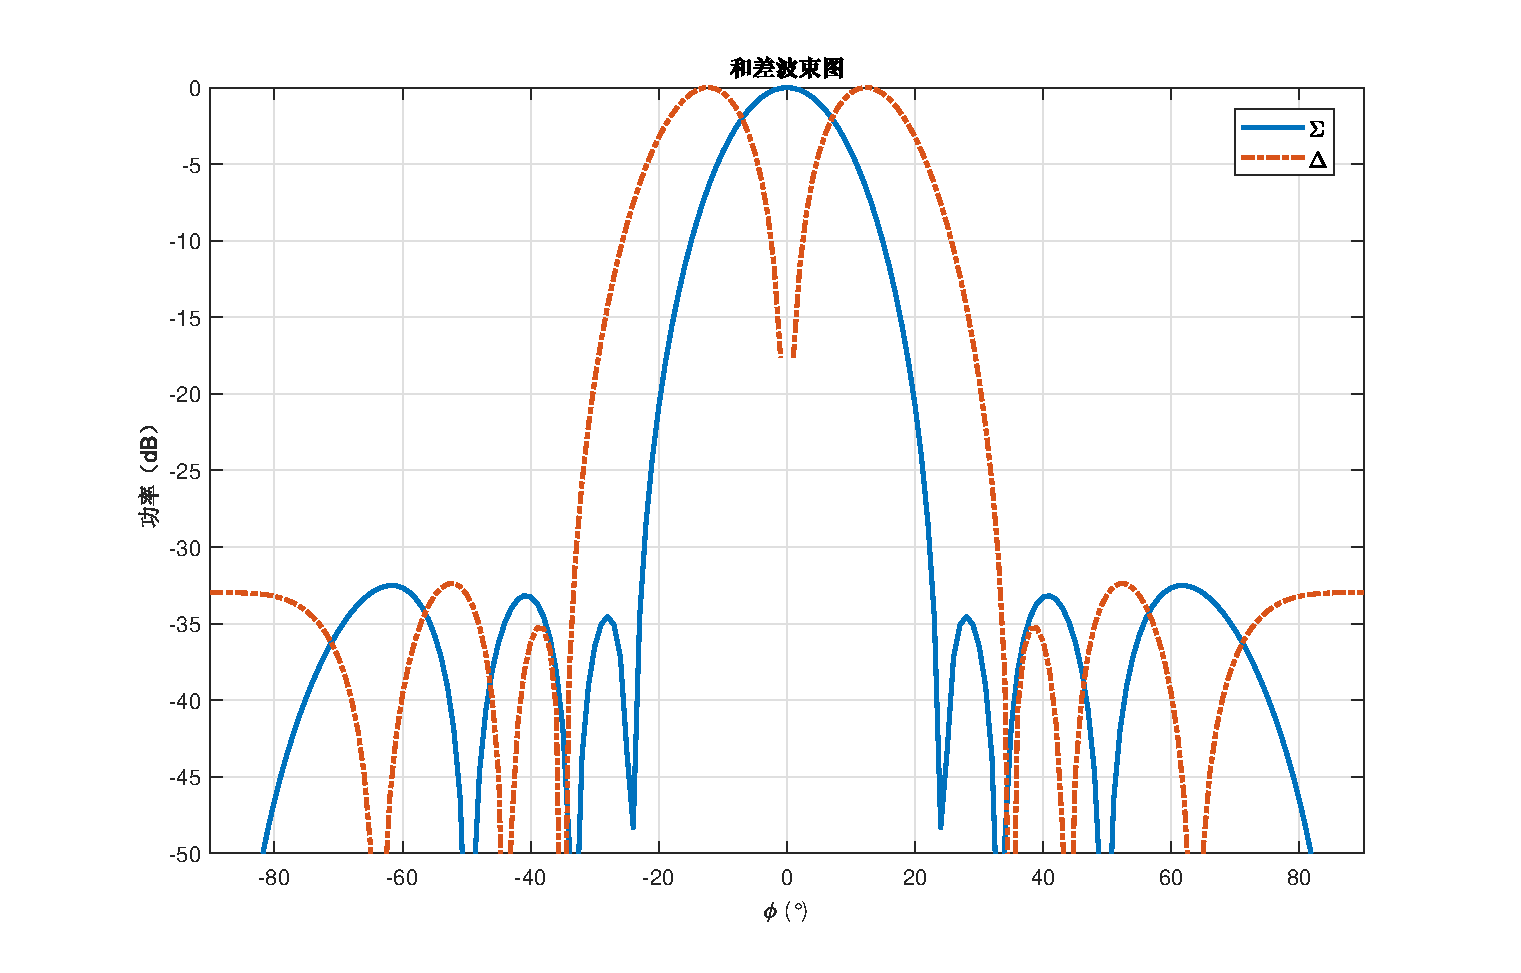
\includegraphics[scale=0.4]{pic/Taylor_Bayliss.eps}
    \caption{Taylor权形成的和波束$\Sigma$与Bayliss权形成的差波束$\Delta$}
    \label{Taylor_Bayliss}
\end{figure}

与半阵法的和差波束图\ref{semi_sigma_delta}相比,加权法得到的和差波束具有更低的旁瓣电平。
这意味着加权法具有更好的旁瓣抑制效果,能够应对存在旁瓣干扰的单脉冲测向场景。
但加窗的步骤使得主瓣展宽,和波束的3dB截止角度此时位于$\pm8^\circ$附近。
另外,加权法的单脉冲比MRC没有显式表达式,我们需要预先对MRC进行线性拟合才能够在单脉冲测向系统中使用它。
图\ref{Taylor_Bayliss_MRC}给出了加权法的单脉冲比曲线。
\begin{figure}[h]
    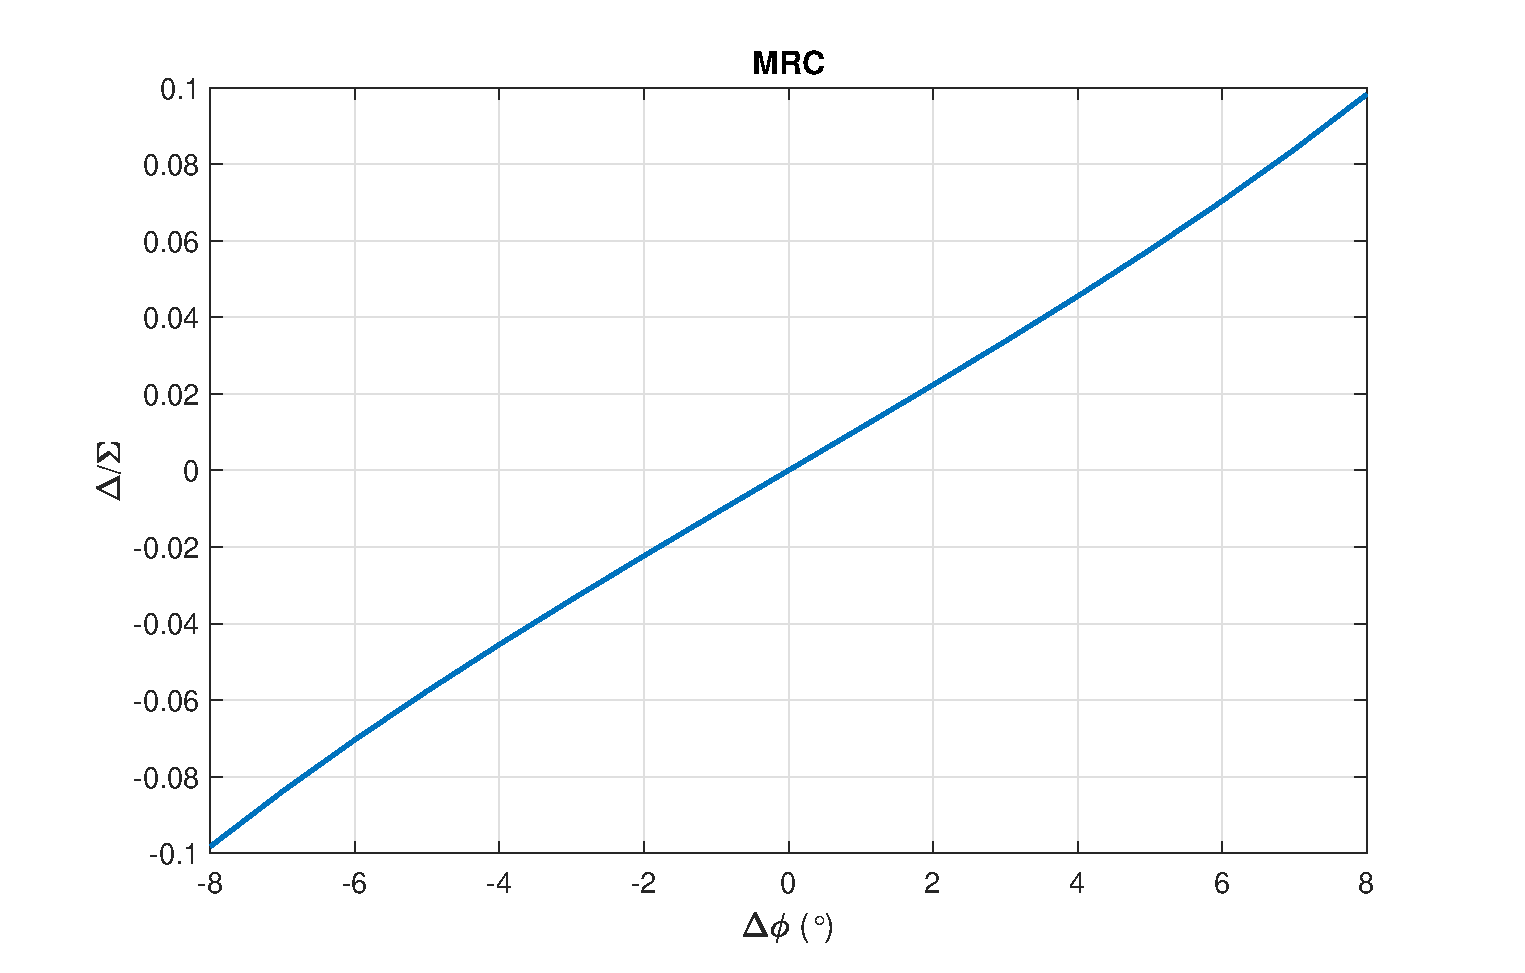
\includegraphics[scale=0.4]{pic/Taylor_Bayliss_MRC.eps}
    \caption{加权法的单脉冲比曲线}
    \label{Taylor_Bayliss_MRC}
\end{figure}

类似的,从图\ref{Taylor_Bayliss_MRC}中可以得知,在远离波束指向$\phi_0$时,MRC的线性度会下降,
从而使得此时的测角误差变大。

\subsection{和差比幅}
半阵法和加权法最大的局限性在于,它们都需要依赖于阵列的特殊结构。
前者要求阵列排布具有对称性,后者只能用于规则阵列且不具普适性,每种不同阵列的权向量表达形式可能会大相径庭。
而本节中将介绍一种名为和差比幅法的单脉冲测向方法。该方法的和差波束形成方式不依赖于阵列结构,
因此可以用于共形阵。

为简化问题,我们依旧以均匀线阵为例来解析和差比幅测向法的一般过程。
首先考虑一个$M$阵元的均匀线阵,阵元间距为半波长,期望信号波长为$\lambda$,阵列波束指向为$\phi_0$。
与半阵法类似,我们首先构造和波束权。由于和波束要求在波束指向处形成主瓣增益,因此我们取波束指向$\phi_0$
处的导向向量作为和波束权,即
\begin{equation}\label{ACM_w_s}
    \begin{aligned}
        \bm{w}_\Sigma = \bm{a}(\phi_0)
    \end{aligned}
\end{equation}
现在构造差波束权。由于差波束要求在波束指向处形成零陷,因此,一种可取的方法是:
首先以波束指向$\phi_0$为中心,关于$\phi_0$对称分别选取两个角度$\phi_l$和,$\phi_r$,
一般情况下,我们选择和波束主瓣的3dB截止角度作为$\phi_l$和$\phi_r$的值;
然后我们将差波束$\Delta(\phi)$构造为两个波束之差
\begin{equation}\label{ACM_delta}
    \begin{aligned}
        \Delta(\phi) = \left|\bm{a}^H(\phi_l)\bm{a}(\phi)\right| - 
                       \left|\bm{a}^H(\phi_r)\bm{a}(\phi)\right|
    \end{aligned}
\end{equation}
同理,比幅法也需要将和波束处理为幅度值,即式
\begin{equation}\label{ACM_sigma}
    \begin{aligned}
        \Sigma(\phi) = \left|\bm{w}_\Sigma^H\bm{a}(\phi)\right|
    \end{aligned}
\end{equation}
最后结合式\eqref{ACM_sigma}与\eqref{ACM_delta},得到比幅法的单脉冲比
\begin{equation}\label{ACM_MRC}
    \begin{aligned}
        \text{MRC} = \frac{\Delta(\phi)}{\Sigma(\phi)}
                   = \frac{ \left|\bm{a}^H(\phi_l)\bm{a}(\phi)\right| - 
                            \left|\bm{a}^H(\phi_r)\bm{a}(\phi)\right| }
                          { \left|\bm{w}_\Sigma^H\bm{a}(\phi)\right| }
    \end{aligned}
\end{equation}
从式\eqref{ACM_MRC}中可以看出,比幅测向顾名思义,是以差波束与和波束的幅度比作为单脉冲比,
实际上利用了左右波束的对称性,而不局限于阵列本身几何结构的特殊性,因此可以用于共形阵。
但该方法受阵列波束特性的影响,比如阵列的主瓣过宽时,可能会导致测向结果较差。
接下来我们仍然通过一个均匀线阵的例子来展示其特性。

考虑一个$8$阵元的均匀线阵,阵元间距为半波长,波束指向$\phi_0=0^\circ$,
我们取$\phi_l=-5^\circ$且$\phi_r=5^\circ$。
此时和差波束如图\ref{ACM_sigma_delta}所示。
\begin{figure}[h]
    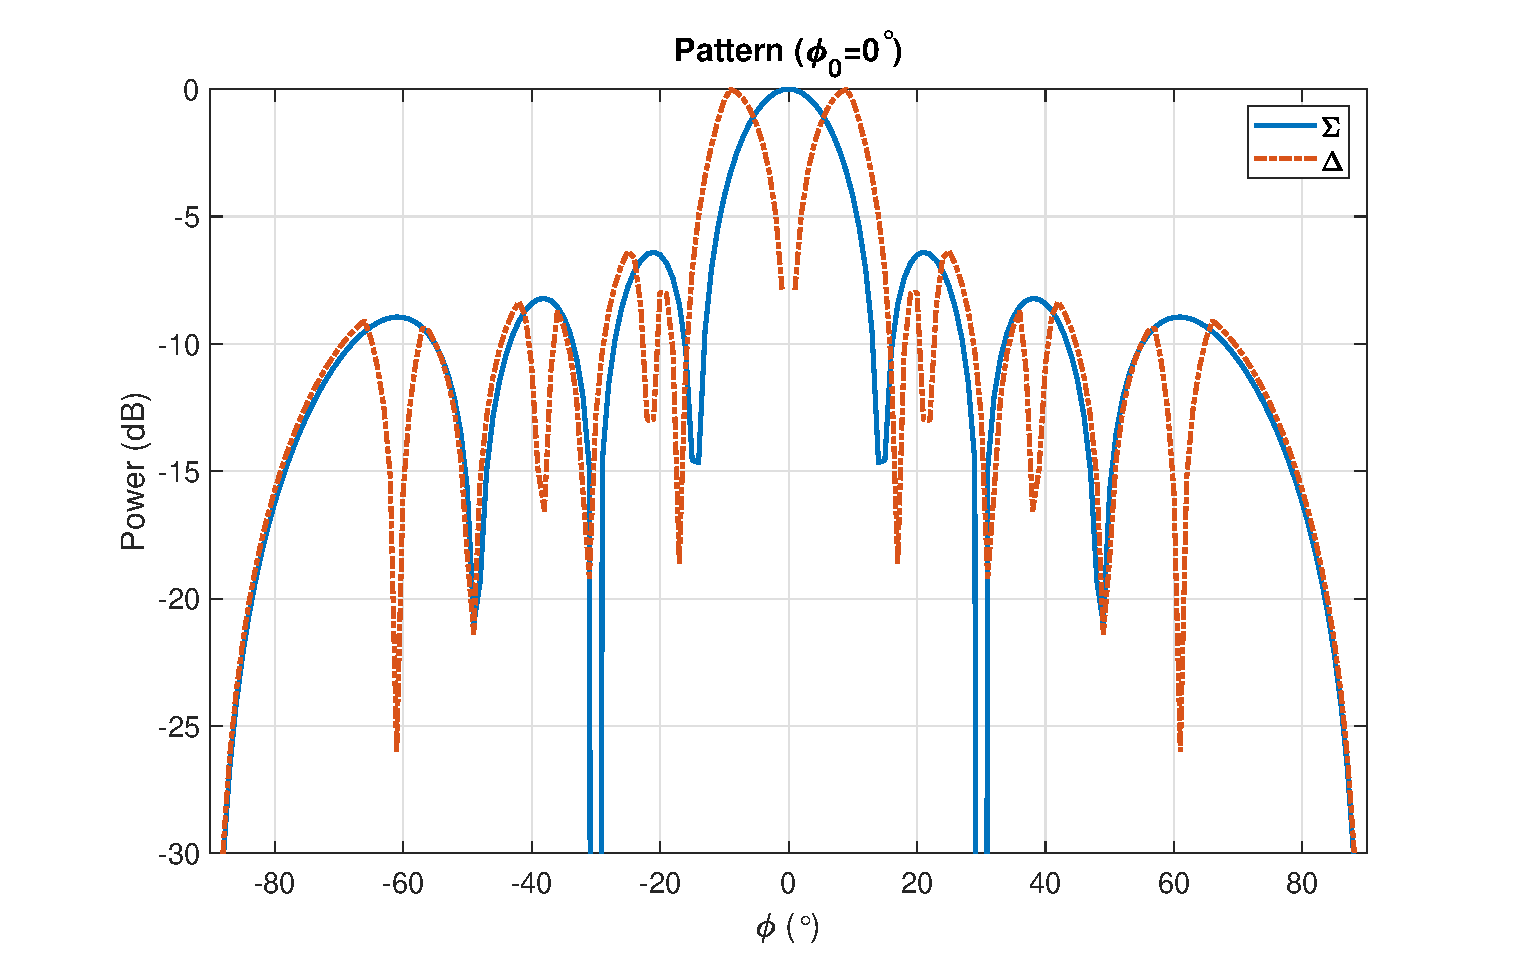
\includegraphics[scale=0.4]{pic/ACM_sigma_delta.eps}
    \caption{比幅法的和波束$\Sigma$与差波束$\Delta$}
    \label{ACM_sigma_delta}
\end{figure}

从图\ref{ACM_sigma_delta}中可以看出,与半阵法类似,比幅法的差波束依然在波束指向$\phi_0$处形成了零陷,
且旁瓣电平较高,难以抑制旁瓣干扰,仍旧无法用于存在强旁瓣干扰的场景。另外,比幅法的单脉冲比MRC也
不存在一个显式表达式,因此只能通过曲线拟合拟合出其斜率,然后在单脉冲测向系统中用于测向。
其单脉冲比曲线如图\ref{ACM_MRC}所示。
\begin{figure}[h]
    \includegraphics[scale=0.4]{pic/ACM_MRC.eps}
    \caption{比幅法的单脉冲比曲线}
    \label{ACM_MRC}
\end{figure}

与之前的两种方法类似,MRC在远离波束指向角$\phi_0$时线性度会下降,进而影响测角精度。

\section{本章小结}
本章中,我们假设组成相控阵的所有阵元天线都是完全一致的全向天线,并给出了相控阵接收信号的数学模型,
进而简要的阐述了波束形成技术和传统单脉冲测向方法。

首先是相控阵的数学模型,依据阵元排布的方式,
我们将其划分为两大类,第一类是规则的阵列主要包含均匀线阵,均匀面阵和均匀圆阵。
我们通过几何光学计算出信号到达各个阵元的波程差,进一步给出其相位差,在远场窄带信号的假设下,
给出了这三种阵列的导向向量。第二类阵列是共形阵,主要特征为其“一般”性,即阵元排布不遵循某一特定规律。
在这种情况下,我们利用信号的方向余弦向量以及每个阵元的笛卡尔坐标计算出信号到达每个阵元的相位差,
进而给出一般导向向量表达式。值得注意的是,第一类规则阵列实际上是共形阵列的一种特殊形式,
其导向向量依然可以根据共形阵导向向量导出。

接着我们介绍了波束形成技术,阐述了波束形成的目的和一般手段。
然后介绍了两种波束形成方法,分别是MVDR方法和LCMV方法。
前者可以保证在设定的指向角$\phi_0$出形成主瓣增益,同时抑制干扰和噪声;
后者则可以在多个指向角同时形成波束和零陷,用于接收信号和抑制干扰。
实际上,MVDR方式是LCMV方法的一种特殊形式,即规定在指向角$\phi_0$处信号无失真通过。
在后续的章节中,我们还将利用LCMV结构进行单脉冲测向。

最后我们给出了三种常用的传统单脉冲测向方法,分别是半阵法、加权法和比幅法,
三种方法的优缺点各异。半阵法主要更近均匀线阵或均匀面阵的对称性,构造出和差波束权向量。
而在单脉冲测向问题中,期望信号的真实方向$\phi_s$往往接近于波束指向$\phi_0$,
因此半阵法利用该特性导出一个关于偏离角$\Delta\phi$的显式线性函数,进一步用于测向过程。
该方法简单易于实现,但依赖于阵列的几何结构,不能用于均匀圆阵和共形阵,
并且其和差波束的旁瓣电平都较高,无法应对有强旁瓣干扰存在时的场景。
因此,T. Taylor和E. T. Bayliss分别提出了一种和差波束加权方法,
进而设计出一种低旁瓣的和差波束权向量。该方法可以用于均匀线阵、均匀面阵和均匀圆阵,
其优点在于底旁瓣的波束能够在一定程度上抑制旁瓣干扰。但加窗的处理过程使得和波束主瓣有一定程度的展宽,
可能会造成测向精度下降,并且这种方法的单脉冲比没有显式表达式,因此只能先进行曲线拟合,
再将拟合好的数据用于后续的单脉冲测向过程。另外,该方法虽然可以拓展至均匀圆阵,
但仍旧无法将其用于共形阵。第三种方法是比幅测向法,该方法通过选取关于波束指向$\phi_0$对称的
两个角度的导向向量来构造差波束,并且单脉冲比直接用差波束与和波束的赋值进行比较,以此测量
偏离角$\Delta\phi$。该方法不受限于阵列结构,可以用于共形阵单脉冲测向。
但该方法与半阵法类似,和波束旁瓣电平仍然较高,无法应对强旁瓣干扰存在的场景。

\chapter{基于旁瓣对消的单脉冲测向方法}
本章中,我们将介绍旁瓣对消波束形成方法及其在单脉冲测向场景中的应用。
旁瓣对消方法通过设置一个阵元个数较主阵列小的子阵列,使得期望信号在该阵列上被阻塞,
而旁瓣干扰可以无阻碍的通过,然后将主阵与子阵输出叠加,以此消除旁瓣干扰。
由于辅助子阵的规模通常小于主阵列,因此该方法减小了计算量。
我们首先介绍旁瓣对消的基本原理,然后给出一种基于拟矩阵和SVD的阻塞矩阵的设计方法,
最后介绍一种正交置零的主瓣干扰消除技术,并结合旁瓣对消,并将其用于单脉冲测向。

\section{旁瓣对消基本原理}
时域积分方程时间步进算法的阻抗元素直接影响算法的后时稳定性,因此阻抗元素的计算是算法的关键之一,采用精度高效的方法计算时域阻抗元素是时域积分方程时间步进算法研究的重点之一。

\section{一种基于拟矩阵和SVD的阻塞矩阵设计方法}
由于时域混合场积分方程是时域电场积分方程与时域磁场积分方程的线性组合,因此时域混合场积分方程时间步进算法的阻抗矩阵特征与时域电场积分方程时间步进算法的阻抗矩阵特征相同。时域阻抗元素的存储技术也是关键技术之一,采用合适的阻抗元素存储方式可以提高并行算法的计算效率。

\section{正交置零主瓣干扰抑制方法}
由于时域混合场积分方程是时域电场积分方程与时域磁场积分方程的线性组合,因此时域混合场积分方程时间步进算法的阻抗矩阵特征与时域电场积分方程时间步进算法的阻抗矩阵特征相同。

\begin{algorithm}[H]
    \KwData{this text}
    \KwResult{how to write algorithm with \LaTeX2e}
    initialization\;
    \While{not at end of this document}{
        read current\;
        \eIf{understand}{
            go to next section\;
            current section becomes this one\;
        }{
            go back to the beginning of current section\;
        }
    }
    \caption{How to wirte an algorithm.}
\end{algorithm}

由于时域混合场积分方程是时域电场积分方程与时域磁场积分方程的线性组合,
因此时域混合场积分方程时间步进算法的阻抗矩阵特征与时域电场积分方程时间步进算法的阻抗矩阵特征相同。
\section{本章小结}
本章首先研究了时域积分方程时间步进算法的阻抗元素精确计算技术,分别采用DUFFY变换法与卷积积分精度计算法计算时域阻抗元素,通过算例验证了计算方法的高精度。

\chapter{相控阵的自适应单脉冲方法}
\section{最大似然方法}
时域积分方程时间步进算法的阻抗元素直接影响算法的后时稳定性,
因此阻抗元素的计算是算法的关键之一,
采用精度高效的方法计算时域阻抗元素是时域积分方程时间步进算法研究的重点之一。

\section{MVAM方法}
时域阻抗元素的存储技术也是时间步进算法并行化的关键技术之一,
采用合适的阻抗元素存储方式可以很大的提高并行时间步进算法的计算效率。

\section{线性约束方法}
由于时域混合场积分方程是时域电场积分方程与时域磁场积分方程的线性组合,
因此时域混合场积分方程时间步进算法的阻抗矩阵特征与时域电场积分方程时间步进算法的阻抗矩阵特征相同。

\section{SVD-线性约束}
如表\ref{tablea}所示给出了时间步长分别取0.4ns、0.5ns、0.6ns 时的三种存储
方式的存储量大小。

\section{本章小结}
结
\chapter{极化相控阵的单脉冲测向方法}

\section{极化相控阵接收信号模型}
本文以时域积分方程方法为研究背景,主要对求解时域积分方程的时间步进算法以及两层平面波快速算法进行了研究。
\subsection{各阵元摆放角度一致的接收信号模型}

\subsection{各阵元摆放角度不同的接收信号模型}

\section{各阵元摆放角度一致的极化相控阵单脉冲测向}
时域积分方程方法的研究近几年发展迅速,在本文研究工作的基础上,仍有以下方向值得进一步研究:

\subsection{原理}

\subsection{性能分析}

\subsection{仿真}

\section{各阵元摆放角度不同的极化相控阵单脉冲测向}

\subsection{原理}

\subsection{仿真}

\section{本章小结}

\chapter{全文总结与展望}

\section{全文总结}

\section{后续工作展望}

\thesisacknowledgement
在攻读博士学位期间,首先衷心感谢我的导师XXX教授

\thesisappendix

\chapter{中心极限定理的证明}

\section{高斯分布和伯努利实验}


% Uncomment to list all the entries of the database.
% \nocite{*}

\thesisbibliography{reference}


% Uncomment following codes to load bibliography database with native
% \bibliography command.

% \nocite{*}
% \bibliographystyle{thesis-uestc}
% \bibliography{reference}

% \thesisaccomplish{publications}

% \thesistranslationoriginal
% \section{The OFDM Model of Multiple Carrier Waves}

% \thesistranslationchinese
% \section{基于多载波索引键控的正交频分多路复用系统模型}

\end{document}
